
\oursection{Implementation}

\oursubsection{DB Loader}
%DB loader is consist of circular ring buffer and large size of memory cache.
DB loader load DB file to large size of ring buffer it has.
It provides internal API for zero-copy read or write on the buffer to search threads.
{\tt acquire(void **ptr, int len)} requests a part of the buffer to read and {\tt release(void *ptr, int len)} releases the acquired part of buffer.
A search thread may hold a part of buffer while searching and releases it after the searching.
DB loader can load another part of DB after a search thread release the buffer it holds on.
Note that GPU search thread may release the buffer before finish searching because it does not need to hold buffer after copying the data to the GPU memory.
%It copies data from or to the buffer when write function or read function is called, respectively.
%In most of cases memcopy is unnecessary and can be replaced by zero-copy read operation.
%The zero-copy operation will be implemented later.
%Large size of memory cache is not implemented yet.
%So DB loader repeatedly reads the DB from disk even when sufficient memory is provided.

\oursubsection{Search Engine}
Search engine is designed to have thread pool of workers, each worker takes some portion of DB from DB loader, and result of each worker is merged together at last.
Unfortunately, current implementation is a bit inefficient.
A portion of DB read by DB loader is divided by 10 pieces and feeded to CPU search threads or GPU search threads one by one.
In CPU search function then spawns worker thread and divide its input to equal pieces for each worker thread.
In GPU search function copies its divided input to GPU and copy the result after processing.
As a result, 1 GB of the DB is divided into too small pieces, 30 MB, so sum of thread creation, data transfer to GPU and other overheads becomes hundreads of milli seconds which is not negligible.

\textbf{AVX:}
Advanced Vector Extension, AVX, is an extended instruction set of x86 provided by Intel to achieve instruction level data parallelism.
CPU can do at most 8 single-precision floating point calculation at once.
Calculating eucladian distance of two different feature vector can be done by only eight iterations of AVX instructions since each feature vector is consist of 64 single-precision floating point variables.

%\textbf{Highly efficient CUDA kernel:}
%Nvidia graphic cards expose L1 cache as shared memory to programmers.
%\note{TBD}

%\textbf{Cache-aware programming:}
%Typical Intel CPUs have 2 or 4 physical cores and 3 to 6 MB of L3 cache shared by all physical cores. \note{Should I delete this paragraph?}

\textbf{Queueing:}
Search engine handles simultaneously incoming requests so it provides circular queue of request and internal APIs for enqueueing.
When there are requests to be processed, they are processed in FIFO order and Search engine sleeps when the queue is empty.

\oursubsection{HTTP Server}

\begin{figure}[t]
	\centering
	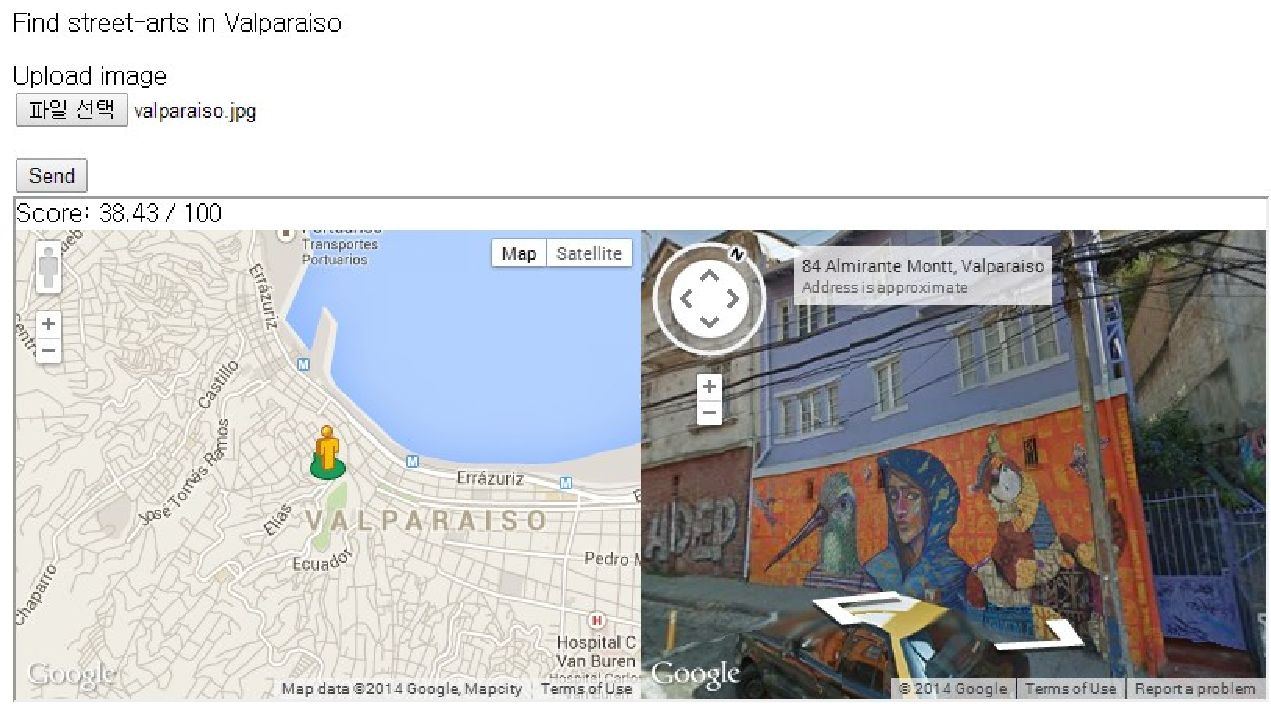
\includegraphics[scale=0.38]{figs/web_sample}
	\vspace{-0.1in}
	\ourcaption{Screen capture of search result web page}
	\vspace{-0.1in}
	\label{fig:web_sample}
\end{figure}

Functionality of HTTP server is divided by two, one is serving front page of the service which includes empty 'iframe' and the other is receive images from a client and update the 'iframe'.
The former is in charge of Nginx, an open source web server, and the latter is in charge of \name{}.
When the client connects to Nginx, it serves a static web page, 'street.html' which has upload button and empty 'iframe'.
When the client uploads an image file, it sends HTTP POST message which has the image file to the \name{}.
HTTP server of \name{} parses HTTP POST message, extract the image and write it to the disk.
Then the HTTP server read it from the disk, SURF it, extract feature vectors, enqueue it to the search engine, and sleep by 'select()' system call.
Limited APIs of OpenCV leads the unnecessary disk access.
Actual disk access may be avoided by using RAM disk.
HTTP server is waken up after the search engine finishes searching.
It sends response html web page, 'resp.html' which include matching score, Google maps and Google street views pointing the location of search result.
Figure~\ref{fig:web_sample} shows an example of the search result web page.
